%% LaTeX2e class for student theses
%% thesis.tex
%% 
%% Karlsruhe Institute of Technology
%% Institute for Program Structures and Data Organization
%% Chair for Software Design and Quality (SDQ)
%%
%% Dr.-Ing. Erik Burger
%% burger@kit.edu
%%
%% See https://sdqweb.ipd.kit.edu/wiki/Dokumentvorlagen
%%
%% Version 1.3.5, 2020-06-26




%% Available page modes: oneside, twoside
%% Available languages: english, ngerman
%% Available modes: draft, final (see README)
\documentclass[twoside,ngerman]{sdqthesis}



%% Name of the author
\author{Oliver Helian Martz}

%% Title (and possibly subtitle) of the thesis
\title{Identifikation von Alternativen zu Einwegverpackungen im Bauwesen}

%% Type of the thesis 
\thesistype{Bachelorarbeit}

%% Change the institute here, ``IPD'' is default
\myinstitute{Institut für Technologie und Management
im Baubetrieb}

%% You can put a logo in the ``logos'' directory and include it here
%% instead of the SDQ logo
% \grouplogo{myfile}
%% Alternatively, you can disable the group logo
\nogrouplogo

%% The reviewers are the professors that grade your thesis
\reviewerone{Prof. Dr.-Ing. Dipl.-Kfm. S. Haghsheno}

%% The advisors are PhDs or Postdocs
\advisorone{Dipl.-Ing. N. Münzl}
%% The second advisor can be omitted
\advisortwo{E. Schwarzweller, M.Sc.}

%% Please enter the start end end time of your thesis
\editingtime{18. 05. 2022}{18. 08. 2022}

\settitle

%% --------------------------------
%% | Settings for word separation |
%% ------------------------

%% Describe separation hints here.
%% For more details, see 
%% http://en.wikibooks.org/wiki/LaTeX/Text_Formatting#Hyphenation
\hyphenation{
% me-ta-mo-del
}

%% --------------------------------
%% | Bibliography                 |
%% --------------------------------

%% Use biber instead of BibTeX, see README
\usepackage[citestyle=numeric,style=numeric,backend=biber]{biblatex}
\addbibresource{thesis.bib}

\usepackage[]{acronym}
%\usepackage[footnote]{acronym} bei fußnote statt einfach so in den text zu schreiben
%von cedric


\begin{document}
%% Set PDF metadata



\setpdf


%% The Preamble begins here
\frontmatter

\maketitle



\thispagestyle{empty}
\null\vfill
\noindent\hbox to \textwidth{\hrulefill} 
\iflanguage{ngerman}{Ich versichere hiermit, dass ich die vorliegende Arbeit selbstständig verfasst habe und keine anderen als die angegebenen Quellen und Hilfsmittel benutzt habe, die wörtlich oder inhaltlich übernommenen Stellen als solche kenntlich gemacht und die Regeln zur Sicherung guter wissenschaftlicher Praxis im Karlsruher Institut für Technologie (KIT) in der aktuell gültigen Fassung beachtet habe.}
 

\textbf{Karlsruhe, den xx.08.22}
\vspace{1.5cm}
 
\dotfill\hspace*{8.0cm}\\
\hspace*{2cm}(\theauthor) 
\cleardoublepage

\setcounter{page}{1}
\pagenumbering{roman}

%% ----------------
%% |   Abstract   |
%% ----------------

%% The text is included from the following files:
%% - sections/abstract

\includeabstract

%% ------------------------
%% |   Table of Contents  |
%% ------------------------
\tableofcontents

\listoffigures
\listoftables

Abkürzungsverzeichnis fehlt noch
Symbolverzeichnis fehlt noch

--> alle verzeichnisse müssen noch ins Inhaltsverzeichns vor die einleitung aber ohne nummerierung--> siehe word vorlage
->sieht auch clean aus

Literaturverzeichnis ans ende ohne nUmmerierung fehlt noch!(vor den anhang)

%% -----------------
%% |   Main part   |
%% -----------------

\mainmatter

\input{sections/Abkürzungsverzeichnis}

\chapter*{Symbolverzeichnis}
\label{sec:Symbolverzeichnis}


Sämtliche im Verlauf der Arbeit verwendete Symbol sollen hier chronologisch aufgelistet werden




\chapter{Einführung}
\label{ch:Einführung}

%% -------------------
%% | Example content |
%% -------------------

\section{Motivation der Themenwahl}
\label{sec:Einführung:Motivation der Themenwahl}

Es geht um die wissenschaftliche Motivation! nicht meine eigene! 

Es ist zu erkennen, dass viele andere Bereiche der deutschen und internationalen Industrie bereits Alternativen zu Einwegverpackungen in Form von Mehrwegverpackungen gefunden haben und sich diese nicht nur durch persönliches Interesse der Geschäftsführung jener Konzerne fundiert, sondern sich die Idee von Mehrwegverpackungen und dauerhaften Alternativen zu Einwegverpackungen auch wirtschaftlich rentiert, sowie ein positives Image der Konzerne als Folge hat.

%Eine meiner Erfahrungen auf einer Baustelle zum Bau eines Einfamilienhauses führte mir nicht nur vor Augen, wie viel Plastik im Allgemeinen Anwendung in der Bauindustrie findet, sondern auch die in meinen Augen häufige Anwendung von Plastiktüten zur Verpackung von Dämmung, sowie die einmalige Nutzbarkeit von Gurten bei der Annahme und dem Anheben von Materialien aller Art durch Einsatz eines Kranes.   






\section{Ziel und Abgrenzung der Arbeit}
\label{sec:Ziel und Abgrenzung}

(Es handelt sich vorrangig um die Frage bzw die Suche nach Mehrwegverpackungen , nur geringfügig nach anderen Arten von Einwegverpackungen(Anhang))
    
Das Ziel dieser Arbeit ist es, eine oder mehrere Alternativen zu Einwegverpackungen im Bauwesen zu finden. Der Operator "Identifikation" gibt an, dass als Ziel dieser Arbeit eine oder mehrere Alternativen zu Einwegverpackungen ermittelt bzw festgestellt werden, diese jedoch (nur als theoretische Grundlage einer ersten Recherche entstanden sind und keinerlei praktische Bestätigung enthalten.)(stimmt das so?)

Inhaltlich steht hierbei die Eignung von Mehrwegverpackungen für typische Bauprodukte und
Baustoffe im Zentrum, sowie eine Erarbeitung von Ansätzen zu Mehrwegverpackungssystemen, die bisherige Einwegverpackungen von Bauprodukten und Baustoffen ersetzen könnten. 

Nicht im Fokus dieser Bachelorarbeit steht das Thema nachwachsende Rohstoffe, die durchaus eine Alternative zu konventionellen Einwegverpackungen wären, jedoch häufig keine ausreichenden Materialeigenschaften haben, um als Mehrwegverpackung angesehen zu werden. Biologisch abbaubare und anderweitig ökologisch sinnvollere Lösungen im Hinblick auf eine Einsprung von CO2 im Lebenszyklus einer Verpackung und der ÖkoBilanz fallen unter selbigen Kriterien nicht in den Fokus dieser Arbeit. (Quelle?)

Die Bereiche des Bauwesens, die für eine Lösung des Problems bzw der Frage in Betracht kommen, sind zusammen mit der Logistik, die Lagerung und ... . Gründe für die Wahl dieser Bereiche sind... . Im Kapitel "Nutzbarkeit von anderen am Markt bereits verfügbaren Systemen für das Bauwesen", wird als Ausnahme hiervon auch die Lebensmittelindustrie und die ... genannt bzw aus ihr referenziert. (Quelle)?

Zuletzt ist eine geographische und rechtliche Abgrenzung auf das Gebiet der Bundesrepublik Deutschland und die hierin geltenden Gesetze notwendig. Die betrifft vor allem das  Verpackungsgesetz(VerpackG) und ...welches dem Erreichen der europarechtlichen Zielvorgaben der Richtlinie 94/62/EG auf Bundesebene (Übernimmt?)

Abgrenzung: 
%-Abgrenzung zu nachwachsenden Rohstoffen:
%-nachwachsende Rohstoffe wie Bio-Kunststoffe (z. B. Maisstärke), Rohrzucker oder Bambus, die biologisch abbaubar sind, kommen vermehrt zum Einsatz.
%-nur Deutschland (bzw nur nach deutschem Vorgehen was Verpackungsgesetze und recycling angeht)
        -->nicht deutsche Möglichkeiten und Ideen sind evtl anders. Kann auch in den Schluss bzw. als eine weitere anschließende Bachelorarbeit-->International-->eher die Staaten anschauen, die am meisten Einwegverpackungsmüll erzeugen-->China, Indien etc.



\section{Methodik}
\label{sec:Einführung:Methodik}

%https://www.scribbr.de/methodik/methodik-schreiben/
Beantworte diese Fragen, wenn du deine Methodik schreibst:
            -ca 10 Prozent der Bachelorarbeit
    
    Welche Art von Forschung nimmst du vor?
        
        -Quantitativ
        -Qualitativ
        -beides(mein Fall)
        -Induktives Vorgehen
            -Wenn du induktiv argumentierst, führst du eine eigene Forschung durch und leitest daraus selbst eine Theorie ab
        -deduktives Vorgehen    
            -Wenn du deduktiv vorgehst, testest du mit deiner Untersuchung eine bereits vorhandene Theorie

Diese Bachelorarbeit ist sowohl qualitativ als auch quantitativ durchgeführt worden. Zur Sammlung von Informationen wurde eine Literaturrecherche durchgeführt, die ... . 

    Wie hast du deine Daten erhoben?
    
        -literaturrecherche + Felduntersuchung:
        -Literaturrecherche bzw Literaturarbeit
            -Datenbanken durchsuchen
            -Berichte analysieren
            -Daten analysieren
            -Metaanalyse durchführen
            -Sekundäranalyse durchführen
            -Diskursanalyse durchführen
            -Quantitative Inhaltsanalyse durchführen

        -quantitative Felduntersuchung:
            -Umfrage durchführen
            -Interviews durchführen
            -Experimente durchführen
            -Beobachtungen mit signifikanten Zahlen durchführen
            -Quantitative Diskursanalyse
            
Um Informationen aus erster Hand aus der Praxis zu sammeln, wurde in dieser Bachelorarbeit ein Interview geführt. 

    Welche Eigenschaften haben deine Daten?
    
    -bei Interview Part:
            -Interviewform festlegen: strukturiert, semistrukturiert, unstrukturiert
            -Zeit und Ort
            -Beschreibung der Interviews
            -%"Um die Zufriedenheit der Kundschaft in Berlin zu untersuchen, wurden am 23. August 2020 semistrukturierte Interviews mit zehn Passanten sowie Passantinnen im Alter zwischen 20 und 50 Jahren in der Nähe der Eisdiele durchgeführt. Es wurden semistrukturierte Interviews gewählt, um geordnete Antworten auf die Teilfragen zu bekommen. So wurde außerdem die Möglichkeit geschaffen auf einige Fragen genauer einzugehen, um mehr Informationen zu erhalten.
            %Die Interviews wurden in einem Raum in der Julianaschule im Julianenweg durchgeführt und dauerten etwa zehn Minuten, wobei die Interviewten nacheinander befragt wurden. Ebenso wurden die Interviews mit dem Einverständnis der zehn Teilnehmenden aufgezeichnet, um die Antworten effektiver analysieren zu können."
            -in deiner Methodik solltest du die Wahl deiner Interview-Fragen begründen
        -bei Literaturarbeit Part:
            -Daten aus:
                -Literatur
                -Datenbanken
                -Anderen Nachschlagewerken
        -Ein- und Ausschlusskriterien
            -im Methodikteil immer angeben, welche Daten du genau verwendet hast:
                -Einschlusskriterien: Welche Daten du in die Untersuchung einbeziehst
                -Ausschlusskriterien: Welche Daten du nicht in deine Untersuchung aufgenommen hast und warum
                    -%"Nur vollständig ausgefüllte Fragebogen wurden in die Untersuchung einbezogen. Des Weiteren wurde die Umfrage nur mit 18-Jährigen durchgeführt, die zum Zeitpunkt der Datenerfassung in Berlin oder Hamburg wohnten. Wenn die Teilnehmenden diese Voraussetzungen nicht erfüllten, wurden ihre Angaben nicht in der Analyse berücksichtigt, weil sie im Rahmen dieser Bachelorarbeit irrelevant sind. 
                    %Inkorrekt ausgefüllte Fragebogen, bei denen unklar war, welche Möglichkeit angekreuzt wurde, flossen nicht in die Auswertung ein, außer wenn die Teilnehmenden konnten im Nachhinein nach der korrekten Antwort gefragt werden konnten."
    
    Wie ist deine Forschung abgelaufen?
        -auf den praktischen Verlauf eingehen
            -z.B.%ob ausreichend Leute auf deine Interviewanfrage geantwortet haben, wie viele es waren, wie viele du interviewt und wann du zufriedenstellende Ergebnisse erhalten hast.
            -Fokussiere dich auf die Rolle des/der Forschenden und die Forschungssituation. Wenn z. B. die Qualität der Interviews negativ beeinflusst wurde, weil im Nebenraum eine Bandprobe stattgefunden hat, kannst du das hier angeben. Reflektiere aber nicht subjektiv den praktischen Forschungsverlauf, sondern bleibe bei der Beschreibung der Fakten.
            
    Wie hast du deine Daten analysiert?
        -Beispielantworten für quantitative Forschung:

            -Statistische Tests
            -Regressionsanalysen
            -Metaanalyse
            -Quantitative Inhaltsanalyse
            -Kombination der genannten Methoden

        -Beispielantworten für qualitative Forschung:

            -Interpretativer oder beschreibender Vergleich von Daten
            -Kodierung und Kategorienbildung von Materialien
            -Qualitative Inhaltsanalyse
            -Untersuchung anhand eines bestimmten Modells, das du in deinem theoretischen Rahmen beschrieben hast
            -Kombination der genannten Methoden

    Sind die Gütekriterien deiner Forschung erfüllt?
        -Bei quantitativer Forschung solltest du darauf eingehen, ob deine Forschung reliabel, valide und objektiv ist.
        -Für qualitative Forschung gelten die Gütekriterien der Transparenz, Reichweite und Intersubjektivität.
        -Möglichkeiten, Gütekriterien zu beschreiben:
            -in einem gesonderten Abschnitt,
            -wenn du die Daten und den Forschungsverlauf beschreibst oder
            -in der Diskussion oder während der Datenanalyse.
    
    -Zeitform der Verben
        -Normalerweise schreibst du den Methodikteil im Präteritum (‚die Zielgruppe war‘) und im Präsens (‚die Daten werden analysiert‘). Falls deine Betreuungsperson angibt, dass sie das Präsens bevorzugt, solltest du dich daran halten (‚die Zielgruppe ist‘).
        -Wenn du auf die Gütekriterien eingehst, verwendest du das Präsens (‚die Forschung ist valide, da …‘). Dabei gelten die allgemeinen Regeln für Zeitformen beim Verfassen einer Bachelorarbeit.


    -Es ist wichtig, dass deine Forschung reproduzierbar ist. Jemand, der dieselbe Untersuchung mit der gleichen Methode durchführt, sollte zu ungefähr denselben Ergebnissen kommen


\section{Aufbau der Arbeit}
\label{sec:Einführung:Aufbau der Arbeit}

Diesen Paragraph ganz am ende ausfüllen, da ich sonst alles immer abändern muss wenn ich die struktur der BA verändere

%%Die Einleitung soll den Leser in die Problematik einführen und das gewünschte Ziel der Arbeit erläutern. Hier kann die Motivation für die Arbeit und eventuell Zusammenhänge, die zur Formulierung der Aufgabe geführt haben dargestellt werden.
%%Dem Leser soll weiterhin die genaue Vorgehensweise zur Problemlösung vorgestellt werden und einen ersten Überblick über die Gliederung der Arbeit gegeben werden. Mit der Einleitung beginnt die fortlaufende Nummerierung der Seitenanzahl.
%%Für den gesamten Text gilt folgende Formatierung:
%	Schriftart: Time New Roman
%	Schriftgröße: 12
%	Zeilenabstand: 1,5
%	Nach Absatz 10pt



\chapter{Definitionen}
\label{ch:Definitionen}



\section{Definition: Einwegverpackung - im Zusammenhang mit
Bauprodukten und Baustoffen}
\label{sec:Definitionen:Einwegverpackung im Zusammenhang mit Bauprodukten und Baustoffen}

Mehrere Definitionen möglich. Daraus meine eigene Definition aufbauen und darauf referezieren.

%(https://packpart.eu/glossar/einwegverpackungen/)
-Eine Einwegverpackung ist eine Verpackung, die für den !einmaligen Gebrauch! bestimmt ist. Diese Verpackung dient oft dem Verkauf eines bestimmten Produktes und ist aufgrund der !Stabilität sowie aus anderen Gesichtspunkten wie Hygiene und Komfort nicht für die Wiederverwendung geeignet!. Nach !einmaligem Gebrauch muss diese Verpackung entsorgt oder dem Wertstoffkreislauf zugeführt werden!.(Einwegverpackung – Definition)

-Die Verpackung hat einen erheblichen Einfluss auf die Höhe der Logistikkosten und die Effektivität von Logistikprozessen(Logistik)
-Einwegverpackungen haben im Überseetransport gegenüber den Mehrwegverpackungen deutliche Vorteile. Das liegt daran, dass sich die Abmessungen von Bauteilen oft ändern und eine Anpassung oder Neuentwicklung einer Mehrwegverpackung unrentabel wäre.(Logistik)
-Verpackungen aus Kunststoff sind wiederverwertbar und gelangen über das Recycling wieder zurück in den Stoffkreislauf, in dem sie als Einweg- oder Mehrwegverpackung wiederbenutzt werden können(Rohstoffe2)

-Die !Rohstoffe! für ihre Herstellung können Pappe, Papier, Kunststoffe wie PET, Polyethylen und andere Arten von Polymeren und nachwachsenden, biologisch abbaubaren Rohstoffen sein.Kunststoffe, Papier, Bambus und Holz. Glas oder Kunststoff

    -!Ansprüchen! an bedarfsgerechte und sichere Lagerung sowie Transport
    -langzeitstabile, hygienische und für Kunden attraktive Verwahrung
    -Ladegut sicher und kostengünstig das Ziel erreichen.
    -hoher Oberflächengüte



Zur eindeutigen Festlegung von wichtigen Begriffen ist eine Definiion häufig verwendeter Begriffe notwendig. Sie bildet zusammen mit dem Kapitel "Abgrenzung der Arbeit" ein Fundament, auf das in dieser Arbeit referenziert wird.
Dazu gehören die Begriffe Einwegverpackung sowie Mehrwegverpackung, als auch der Begriff Packmittel, der als übergeordneter Begriff jegliche Art von Verpackungen abdeckt. Hinzu kommen die beiden Begriffe Bauprodukte sowie Baustoffe.   




%Thema: Minimierung von Plastikabfällen auch mein Thema?
%Thema: biologisch abbaubare Verpackungen als Teil meiner BA?
%-->(https://packpart.eu/glossar/einwegverpackungen/(Ökologische Einwegverpackungslösungen))




\section{Definition: Mehrwegverpackung - im Zusammenhang mit
Bauprodukten und Baustoffen}
\label{sec:Definitionen:Mehrwegverpackung im Zusammenhang mit Bauprodukten und Baustoffen}

(%https://packpart.eu/glossar/einwegverpackungen/)
-Im Gegensatz zu Einwegverpackungen bestehen Mehrwegverpackungen aus langlebigen und wiederverwendbaren Materialien, die im Alltag oder in der Produktion mehrfach verwendet werden können.(Einwegverpackung – Definition)


%(https://packpart.eu/glossar/mehrwegverpackung/)
Definition: Mehrwegverpackung: 
-Verpackung, die zum mehrmaligen Gebrauch bestimmt ist. Wiederverwendung nach Reinigungs- und Aufbereitungsprozess. Der Lebenszyklus beträgt oft mehrere Jahre. 
-Unterschied zur Einwegverpackung: hauptsächlich die Dauer des Lebenszyklus(aufgrund stabilierer Verarbeitung)


-Begriff Umlauf:(wie häufig etwas wiederverwendet werden kann-->Indikator)
-Mehrwegverpackung Beispiele
    Gitterboxen
    Europaletten -->Beladung, Auslage und Vertrieb
    Kunststoffboxen
    Mehrwegflaschen
    Getränkekisten
    Joghurtgläser
-Umsetzung und Organisation eines Mehrwegsystems(-->Indikator)
-Gesetzliche Vorgaben-->Indikator
-umweltfreundliches Image -->Indikator
-Begriff: Tertiärverpackung(Transport und Lagerung)
-Lagerung der Mehrwegverpackungen(zb Stapeln)-->Indikator
-Mehrwegverpackungen sind besonders gut für sperrige und schwere Packgüter


-Kriterien für die Wahl eines Verpackungsmaterials:(v.a. für den optimalen Schutz) %(https://packpart.eu/glossar/packmittel/)
    -Transport: Bei der Wahl des Packmittels ist sicherzustellen, dass die Produkte auf dem Transportweg dank des Packmittels gut geschützt werden. Zum Beispiel muss per Luftfracht transportierte Ware atmosphärischen Veränderungen und Turbulenzen standhalten.
    -Feuchtigkeit: Zu feuchte Umgebung beim Transport und bei der Lagerung der Produkte kann zu erheblichem Qualitätsverlust führen. Die richtige Verpackung schützt vor Feuchtigkeit.
    Produkteigenschaften: Wertigkeit, Zerbrechlichkeit, Produktgröße sowie Gewicht sind wichtige Faktoren bei der Auswahl der richtigen Packstoffe.
    -Temperatur: Die gewählte Verpackungslösung muss den Produkten eine optimale thermische Umgebung bieten. Dies gilt insbesondere bei verderblichen Produkten wie Lebensmittel.
    Es gibt viele Packmittel auf dem Markt. Dabei hat jedes Material seine Vor- und Nachteile.

-Begriff: Primär-, Sekundär- und Tertiärverpackungen %https://packpart.eu/glossar/packmittel/
    = hierarchische Reihenfolge der Produktverpackungen
    -Primär:
        -umhüllt das eigentliche Produkt und hat das Ziel, optimale Bedingungen für die Lagerung der Produkte zu schaffen
    -sekundär:
        -keinen direkten Kontakt mit der Ware und hält oft mehrere Primärverpackungen zusammen
        -Ziel: Schaffung der Kompaktheit und eines leichten Transports
    -tertiär:
        -vereint die sekundär verpackten Produkte und ermöglicht einen sicheren Transport in sehr großen Produktmengen (Paletten)


\section{Definition: Bauprodukt und Baustoff}
\label{sec:Definition: Bauprodukt und Baustoff}

    -Bauprodukt
            %https://eur-lex.europa.eu/legal-content/DE/TXT/?uri=CELEX:32011R0305
           [Der Ausdruck Bauprodukt bezeichnet] jedes Produkt oder jeden Bausatz, das beziehungsweise der hergestellt und in Verkehr gebracht wird, um dauerhaft in Bauwerke oder Teile davon eingebaut zu werden, und dessen Leistung sich auf die Leistung des Bauwerks im Hinblick auf die Grundanforderungen an Bauwerke auswirkt" aus VERORDNUNG (EU) Nr. 305/2011 DES EUROPÄISCHEN PARLAMENTS UND DES RATES vom 9. März 2011, KAPITEL I, Artikel 2, 1. Absatz (Bauproduktengesetz)
           
           %https://link.springer.com/content/pdf/10.1007/978-3-8348-9919-4.pdf
           Bauprodukte im Sinne des BauPG sind 
                1. Baustoffe, Bauteile und Anlagen, die hergestellt werden, um dauerhaft in bauliche Anlagen des Hoch- oder Tiefbaus eingebaut zu werden, 
                2. aus Baustoffen und Bauteilen vorgefertigte Anlagen, die hergestellt werden, um mit dem Erdboden verbunden zu werden, wie Fertighäuser, Fertiggaragen und Silos.
                
                Eine Besonderheit der Bauproduktenrichtlinie besteht darin, dass die wesentlichen Anforderungen nicht in Bezug auf das Bauprodukt selbst, sondern in Bezug auf das Bauwerk formuliert werden. Für die Anwendung der BPR sind deshalb weitere über den Richtlinientext hinausgehende Erläuterungen erforderlich; hierzu zählen die Grundlagendokumente und die Leitpapiere.
        
                    -Nach §3 Abs. 2 MBO dürfen Bauprodukte „nur verwendet werden, wenn bei ihrer Verwendung die baulichen Anlagen bei ordnungsgemäßer Instandhaltung während einer dem Zweck entsprechenden angemessenen Zeitdauer die Anforderungen dieses Gesetzes oder aufgrund dieses Gesetzes erfüllen und gebrauchstauglich sind.“
                    %https://link.springer.com/content/pdf/10.1007/978-3-8348-9919-4.pdf
            
            wesentlichen Anforderungen:(von Bauprodukten bzw eher Bauwerken, nicht von verpackungen)%-->diese müssen jedoch durch die verpackung erhalten bleiben!!!
                1. Mechanische Festigkeit und Standsicherheit
                2. Brandschutz
                3. Hygiene, Gesundheit und Umweltschutz
                4. Nutzungssicherheit
                5. Schallschutz
                6. Energieeinsparung und Wärmeschutz
            
            
        ( %http://www.derbrandschützer.de/2017/03/25/was-ist-eigentlich-ein-bauprodukt/
            Vereinfacht: Bauprodukte = Produkte, Baustoffe, Bauteile oder Bausätze
            
            Kriterien von Bauprodukten: 
                    -werden hergestellt oder als Anlage vorgefertigt
                    -werden dauerhaft in bauliche Anlagen eingebaut oder als vorgefertigte Anlage mit dem Erdboden verbunden
                        Beispiel:
                        -abnehmbaren Ausschmückungen oder bewegliche Ausscmückungen sind keine Bauprodukte (da nicht dauerhaft in bauliche Anlagen eingebaut
                        -festmontierter „Einbauschrank“ hingegen, könnte bei dieser Definition aber ggf ein Bauprodukt sein. laut alter vorordnung wäre der einbauschrank ein bauprodukt, laut neuer nicht
                    -wirken sich auf die Allgemeinen Anforderungen aus, die nach § 3    MBO 2016 an bauliche Anlagen gestellt werden
                        -Ein Bauprodukt muss sich zudem auch auf die allgemeinen Anforderungen, die nach § 3 MBO 2016 an bauliche Anlagen gestellt werden, „positiv“ auswirken:
                        -§ 3 Allgemeine Anforderungen:
                            "(1) Anlagen sind so anzuordnen, zu errichten, zu ändern und instand zu halten, dass die öffentliche Sicherheit und Ordnung, insbesondere Leben, Gesundheit und die natürlichen Lebensgrundlagen, nicht gefährdet werden; dabei sind die Grundanforderungen an Bauwerke gemäß Anhang I der Verordnung (EU) Nr. 305/2011 zu berücksichtigen.")
            
    -Baustoff:   ----> hierzu gibt es keine wirklichen definitionen
            wikipedia sagt: %https://de.wikipedia.org/wiki/Baustoff
                    -Ein Baustoff ist ein Material (in Form von Rohstoffen, Bauhilfsstoffen oder Halbzeug), das zum Errichten von Bauwerken und Gebäuden benutzt wird. 
                    - In der gesetzlichen Nomenklatur werden Baustoffe als Bauprodukt bezeichnet.
                    

\section{Definition Packmittel}
\label{sec:Definitionen:Definition Packmittel}

-!Begriff Packmittel!: (%https://packpart.eu/glossar/packmittel/)
    -Verpackung eines Produktes zu verstehen und bezieht sich auf Materialien, Gegenstände bzw. Vorrichtungen, die zur Lagerung, Handhabung, Transport, Präsentation sowie zum Schutz von Waren verwendet werden. Packmittel werden im gesamten Kreislauf integriert, angefangen vom Rohstoff bis zum Endprodukt, vom Hersteller bis zum Endverbraucher.
    -Arten von Packmitteln: Handels-, Sammel- und Transportverpackungen...(hierzu gibt es ganze kapitel)
    -Zweck von packmitteln:
        -Schutzfunktion
        -Prozessoptimierung
        -Optimierungsfunktion
        -Erleichterung der Buchhaltung
        -Nutzungsoptimierung
        -Informationsfunktion
    -Packmittelmaterial:
        -Metall
            -aus dünnem Metall:     -flexibel in der Handhabung
                                    -sehr widerstandsfähig
                                    -anpassungsfähig für verschiedene Zwecke
                                    -wird häufig als Rückverpackung verwendet(zb Faltständer und Stahlregale)
                                    -langlebig
                                    -guter Schutz der Produkte vor Erschütterungen während des Transports und grobem Umgang
                                    -Nachteil:  -Möglichkeit einer Korrosion
                                                -massives Gewicht
                                                
        -Kunststoff:    -universell
                        -nützlich für Einzelhandel und Transportwege
                        -geringen Gewicht
                        -Festigkeit
                        -langlebigkeit
                        -einfacher Reinigung
                        -guter Schutz vor mechanischen Schäden
                        -verhinderung von Eindringen von Staub
                        -feuchtigkeitsbeständig
                        -Nachteil:  -Entsorgen der Kunststoffverpackungen
                                    - damit verbundenen Auswirkungen auf die Umwelt
                                    
        -Wellpappe:     -geringen Kosten -->deshalb beliebt
        (=Karton?)      -leicht anpassbar an Form und Größe
                        -guter Schutz
                        -Nachteil:  -Keine große Widerstandsfähigkeit gegen
                                        -mechanische Einwirkung
                                        -Feuchtigkeit
        -Holz       -sicher
                    -gut für:   -große Produkte
                                -schwere Lasten
                                -Komplexe Lasten
                    -langfristige Lagerung gut möglich
                    -Nachteile:     -Sperrigkeit
                                    -geringe Flexibilität
        -Karton
        -Folie
         (=Kunststoff?)             
            
        Kriterien:  -abhängig vom Produkt(Gewicht, Größe, Beschaffenheit, Transportart
                    -Kosten(Logistikkosten,...)
                    -Lagerung
                    -Handhabung
                    -Transport
                    -Präsentation
                    -Schutz der Ware














\chapter{aktueller Praxisstand von Verpackungen}
\label{sec:aktueller Praxisstand von Verpackungen}

\section{Aktueller Praxisstand zum Einsatz von Mehrwegverpackungen und anfallendem Einwegverpackungsmüll auf Baustellen}        
\label{sec:aktueller Praxisstand von Verpackungen:Aktueller Praxisstand zum Einsatz von Mehrwegverpackungen und anfallendem Einwegverpackungsmüll auf Baustellen}


    -Mehrwegverpackungssysteme im Bauwesen: (aus der Sicht eines Bauunternehmers-Rohbau)
    (Daniel Wagner)
        -europaletten
        -pfandpaletten
        -verschiedene paletten für verschiedene steine. mit pfandsystem
        -gitterboxen/euroboxen für rohre, loses material,für kleinere Steine.
        -big pack's? überwiegend schüttmterial- kies, sand, ziersplit.
                -warum keine container?
                    -wegen kosten für die anfahrt, abfahrt und miete und der größe, da containerhäufig zu groß sind. Noch größere mengen werden sonst auf dem lkw oder dem container geliefert.
                -werden jedoch nicht immer wiederverwendet.
        -klebeschaum, dämmschaum muss wieder abgeben werden bzw die leeren Behälter davon. ist jedoch kostenlos. 
        -wird meist mit dem Kran angehoben, oder stapler.(meist jedoch Kran)
            -beim einfamilen haus und mehrfamilien hausbau ist immer ein kran da. es wird fast alles meist mit dem lkw geliefert, die einen kran am start aben und das dann abladen.
        
        --->Ideen dazu: 
                -Pfandsystem auch auf andere Maustoffe umlenken (bzw Verpackungssysteme)
                -zu den einzelnen Punkten ggf. noch weiter recherchieren. je nach Wichtigkeit

------------------------------------------------------------------------------------------

Daniel Wagner über seinen quantitativen "Verbrauch"

        -wie viel ist bisher einwegverpackungsmüll auf deiner Baustelle? (in [t] oder %)
        
            --dämmung in m³   1.5-2 tonne styropor und styrodur (pro einfamilienhaus)
                -Kosten bei Entsorgung: Styrodur -Abfälle ca. 260-280 Euro
            --plastikabfall: 10-15m³ verpackungsfolie, bänder für steine etc
                -Kosten: 135 Euro die Tonne
            --Einwegbänder: 0.5-1 m³
                -Stahl kommt mit einwegbändern. früher war mit Draht verbunden, dann kam eine Gesetzesänderung
                    -Stahlabfälle kostenlos
                -Einmalbänder ca 4 Euro im Einkauf. 
                -beim Einkauf ca 500-600 Euro pro Einfamilienhaus+ Entsorgung 
                -früher sind die steine mit Flachstahlbändern fixiert werden. 
                    -diese waren wiederverwertbar. es ist möglich, alles zurückzugeben, kostet aber meistens mehr und landet z.B. bei Yttong auch auch der Müllhalde.
        -Größenordnung wichtig: Einfamilienhausbau vs größere Baustellen
            -seiner Meinung nach unterschiedlich? 
                    -wenn ja inwiefern?
                        --dämmung wird geringer bei größeren gebäuden. 
                        --wird aber immer gleich geliefert.
                        --steinwolle und holzwolle auf ner palette eingeschweßt in folie
                        --ca 100m" mineralwolle pro
                        --folie wichtig, da sonst wasser zieht
                        --mineralwolle/steinwolle ist feuerfest und brand. AVR.
                        --holzwole für das dach
                        --steine auf paletten mit bändern.
                        --Porenmeton(yttong) muss eingescheißt werden, weil es wasser zieht. 





------------------------------------------------------------------------------------------

Anfallender Verpackungsmüll auf der Baustelle:

Vorgang von Abfällen:   -Transport der Abfälle zu Sammelbehältern
                        -getrennte Sammlung
                        -Abtransport
                        -entsprechende Transportwege, Lagerflächen und Stellflächen
    -Kreislaufwirtschaftsgesetz (KrWG): 
        definiert Abfälle als Stoffe oder Gegenstände, deren sich der Besitzer
        entledigt, entledigen will oder entledigen muss. Das KrWG gilt insbesondere für Erzeuger und Besitzer von Abfällen, für Einsammler oder Beförderer von Abfällen sowie für Unternehmen, die Abfälle in einem Verfahren nach Anhang II KrWG entsorgen.
    Unterschieden in:
    - Abfälle zur Verwertung und
    - Abfälle zur Beseitigung.
    außerdem unterschieden in:
    -gefährliche Abfälle (wenn durch § 48 Satz 2 KrWG „durch Rechtsverordnung be-
        stimmt worden sind“
    -nicht gefährliche Abfälle
    
Oberbegriff für alle Abfälle, die bei Bauarbeiten jeglicher Art anfallen, lautet Bauabfälle. 
        -->Unterpunkt Verpackungsabfälle: 
                        "Zu Verpackungsabfällen zählen Verkaufs- und Transportverpackungen von Bau- und Bauhilfsstoffen aus unterschiedlichen Materialien wie z. B. Kunststoffen."

Umgang mit Abfällen:
    aus rechtlichen und wirtschaftlichen Gründen eine Grundtrennung des Abfalls vorgenommen werden. Die dafür notwendigen Maßnahmen hängen vom anfallenden Abfall in Art, Geometrie und Menge, vom Bauablauf und von den Platzverhältnissen auf der Baustelle ab.

Mögliche Trennung von Verpackungsmüll trennen nach:
        Papier-Verpackungen, Styropor-Verpackungen, Folien-Verpackungen, Kunststoff-Umreifungen, Kunststoffgebinde (Fässer, Kanister usw.).
    -Aus dem Bereich der Verpackungen sollten auf allen Baustellen zunächst Folien, Pappe, Papier und Papiersäcke als wesentliche Verpackungsabfälle getrennt gesammelt werden.

Wichtige Vorschriften und Regeln:

    Kreislaufwirtschaftsgesetz (KrWG)
    Abfallverzeichnisverordnung (AVV)
    Gewerbeabfallverordnung (GewAbfV)
    DIN 18 459 VOB Vergabe- und Vertragsordnung für Bauleistungen - Teil C: Allgemeine Technische Vertragsbedingungen für Bauleistungen (ATV) - Abbruch- und Rückbauarbeiten
    
    Für jede Abfallart muss in der Regel ein Behälter vorgesehen werden. Die Wahl des Sammelbehälters sollte in Absprache mit dem beauftragten Entsorger erfolgen, um den günstigsten Entsorgungsweg zu ermöglichen.

-->wichtig hierbei: Zu Verpackungsabfällen zählen nur Verkaufs- und                                        Transportverpackungen!  

--------Quelle Ende--------



Abfall:

    %(https://www.sanier.de/entsorgung/abfallarten)
    Abfallarten auf der Baustelle:
        -vier verschiedene Kategorien:  -Siedlungsmüll, 
                                    -Sonderabfälle
                                    -Wertstoffe 
                                    -Verpackungsabfälle
            --> nur zum Teil zutreffend
                -->deshalb speziellere Unterteilungen von der Berufsgenossenschaft Bau (BG    Bau)
                -->einzelnen Abfallarten haben jeweils besondere Entsorgungsregelungen
        Andere Unetrteilung:
        -nichtmineralischen Materialien der Bautätigkeit:
        -Bauschutt (besteht aus vorwiegend mineralischen Bestandteilen)
    


Entsorgung:

    %(https://www.interseroh.de/fileadmin/PDF/Broschueren_und_Informationsmaterial/Merkblatt_zur_Entsorgung_von_Transportverpackungen.pdf)
    aktueller Stand von !Entsorgung! von Transportverpackungen(eines Unternehmens(beispielhaft))
        -Verpackungsarten:  -Papier, Pappkarton, Wellpappe mit Polsterung
                            -Folien, PE-Schrumpf-, Stretch- und Luftpolsterfolien
                            -PE-Schaumstoffverpackungen (unvernetzt)
                            -PUR-Schaumstoffverpackungen
                            -Umreifungsbänder aus Kunststoff
                            -Umreifungsbänder aus Stahl
                            -Paletten und Verpackungen aus Massivholz
                            -Paletten und Verpackungen aus Holzwerkstoffen
                            -EPS (z.B. Styropor®)
                            -Papiersäcke und -beutel sowie Verbundsäcke und -beutel (Baustoffsäcke)
                            -PE- und PP-Eimer, -Dosen, -Kartuschen, -Hobbocks, -Kanister und -Fässer
                            -Weiß- und Schwarzblecheimer, -Dosen, -Kartuschen, -Hobbocks, -Kanister und -Fässer

        -Art der Behälter/Erfassung:
                            -Wechselbehälter
                            -Umleerbehälter
                            -Sammelsäcke
                            -lose Erfassung


Duales System Deutschlands(DSD) und der grüne Punkt!!!!!!!!!




Stoffkreislauf von Einwegverpackungen als Thema?
    -->(Lebenszyklus)




%https://www.mt-metallhandwerk.de/bauabfaelle-vermeiden-sortieren-wiederverwerten-27112020
Tausch- oder Restebörsen
    -bei einem Projekt übrig gebliebene:
        -Stahl-/Metallprofile, Lack-, Isolier-, Dämmmaterial- oder Folienreste
        
Was fordert die Gewerbeabfallverordnung? 
    Für folgende zehn Abfallkategorien (Fraktionen) der Bau- und Abbruchabfälle sieht die GewAbfV eine Getrenntsammlung vor: Metalle, Dämmmaterial, Kunststoffe, Baustoffe/Gips, Holz, Glas, Beton, Bitumen, Fliesen/Keramik und Ziegel. 

Hersteler fürchten durch Transport- und Lagerschäden bedingte Reklamationen
    -->deshalb verwenden sie so viel einwegverpackungen
    
Schutt, Abfall oder Sondermüll?
Da die Entsorgungskosten für Baumischabfall deutlich höher sind als für Bauschutt, werden beim Rückbau vor dem eigentlichen Abriss möglichst viele Stoffe, die nicht zum Bauschutt gehören, entfernt.
    -Zum Bauschutt gehören alle mineralischen Stoffe, wie Sand, Backsteine, Natursteine, Mörtel, Putz, Dachziegel, Beton, Zement, Estrich, Sanitärkeramik, Fliesen, Kacheln oder Feinsteinzeug. 
    -Baumischabfälle sind Gläser, Glasbausteine, Bauholz, Metall und Schrott, Gipskarton und Tapeten, Porenbeton, Kabel und Rohre, Dämmstoffe, Isolierungen, Türen und Fenster, Verpackungen und Kunststoffe. 
    -Zum Sondermüll gehören Materialien, die Schadstoffe enthalten, zum Beispiel PCB-haltiges Altholz, Lackreste, Bauschaumdosen, Schamottsteine oder Asbestzementplatten. 
    
------------------------------------------------------------------------------------------------------

VDI 4460 (2003-03-00) März 2003 - Inhaltlich überprüft und unverändert weiterhin gültig: Dezember 2012
Mehrwegtransportverpackungen(MTV) und Mehrwegsysteme zum rationellen Lastentransport
%https://perinorm-s.redi-bw.de/perinorm/fulltext.ashx?fulltextid=20ecb68d7b544a98b63cff8991485f05&userid=1a37bae9-63b1-4cef-8afa-a5709d199868

aktueller Praxisstand: (bzw möglichkeiten, die es im Mehrwegverpackungs-Bereich im bauwesen gibt)
    
    Grundformen der Mehrwegladungsträger:
        -Hauptgruppen der Mehrwegladungsträger:
            -Mehrwegladungsträger mit tragender Funktion (z.B. Flachpaletten)
            -Mehrwegladungsträger mit tragender und umschließender Funktion (z.B. Boxpaletten, Paletten mit Aufsetzrahmen, Rungenpaletten)
            -Mehrwegladungsträger mit tragender, umschließender und abschließender Funktion (z.B. Tankpaletten, IBC)


\section{Anforderungen und Eigenschaften von Verpackungen im Bauwesen}
\label{sec:Anforderungen und Eigenschaften von Verpackungen im Bauwesen}

%https://www.medewo.com/blog/de/loesungen/was-muss-eine-verpackung-leisten/
Was muss eine Verpackung leisten? Unsere Antwort: Den Wert der Ware erhalten!


\subsection{Vor- und Nachteile von Einwegverpackungen}
\label{sec:Vor- und Nachteile von Einwegverpackungen}


%https://packpart.eu/glossar/einwegverpackungen/
Vor und Nachteile von einwegverpackungen:
-Vorteile:
--> -höhere Wirtschaftlichkeit durch günstige und leichte Herstellung
    -Individualisierbarkeit des Designs
    -vereinfachte Lagermöglichkeit
    -Gewährleistung der Transportsicherheit
    -Erfüllung von gesetzlichen und hygienischen Vorschriften
            %(https://www.bmuv.de/faqs/mehrwegverpackungen/)
        -->allgemeinen Hygienevorschriften nach der VO (EG) Nr. 852/2004
        --> Auswahl bei Ausgabe von Mehrwegverpackungen auf ein geeignetes, als sicher anerkanntes Lebensmittelkontaktmaterial achten
            --> keine Verantwortung für die Eignung und Beschaffenheit des Behältnisses für Lebensmittel oder Getränke in vom Kunden mitgebrachte Dosen oder Becher
    -hohe Attraktivität für Endverbraucher durch einfache Handhabung
    (-Geringes Gewicht: spart geld bei transport und gut für unterwegs(bei flaschen))

-Nachteile:
-->schlechtere Umweltverträglichkeit
-->Ökobilanz (besseren CO2-Fussabdruck(oder ist das eigener Punkt?))


\subsection{Vor- und Nachteile von Mehrwegverpackungen}
\label{sec:Vor- und Nachteile von Mehrwegverpackungen}


Vorteile der Mehrwegverpackungen:
%(https://packpart.eu/glossar/mehrwegverpackung/)
-mehrmalige Nutzung
-(nachhaltigen Umgang mit Ressourcen(einmaliger Aufwand zur Herstellung))
-    Robustheit
    weniger Abfall, durch mehrmalige Verwendung
    ressourcenschonender als Einwegverpackungen  
    kleinerer CO2-Fußabdruck bei der Herstellung
    Nachhaltigkeit als Image des Unternehmens
-Kosten:häufig hohe Erstbeschaffung, aber mittel- bis längerfristig billiger
-Umweltfreundliche Aspekte: Müllreduzierung, Ressourcenschonung, CO2-Bilanz(Vermeidung einer Vielzahl der Strecken, die in der Produktion per LKW transportiert werden -->Produktionskette)
- deutlich höheren Schutz der Produkte, besonders bei widrigen Wetterbedingungen wie Regen oder Schnee%(https://www.ecosistant.eu/mehrwegverpackungen-vorteile-nachteile/)


Nachteile Mehrwegverpackungen %(https://packpart.eu/glossar/mehrwegverpackung/)
-eventuelle Probleme mit der Hygiene bei der Aufbereitung und Wiederbefüllung 
-bei Änderung des Verpackungsdesigns sind Flaschen mit altem Design noch lange im Umlauf


------------------------------------------------------------------------------------------

\section{Auswirkungen und Möglichkeiten im Rahmen des Verpackungsgesetzes in Bezug auf nachhaltige Veränderungen im Bauwesen}
\label{sec:Definitionen:Auswirkungen und Möglichkeiten des Verpackungsgesetzes in Bezug auf potentielle Änderungen im Bauwesen}

-Gesetzlicher Rahmen:

%(https://www.verpackungsgesetz.com/)
Verpackungsgesetz (VerpackG):
    "deutsche Umsetzung der europäischen Verpackungsrichtlinie 94/62/EG (kurz PACK) zur Regelung des Inverkehrbringens von Verpackungen sowie der Rücknahme und Verwertung von Verpackungsabfällen."
    -ersetzt seit 03.06.21 den Vorgänger "Verpackungsgesetz 1"(VerpackG1)
      -gilt nur in der Bundesrepublik Deutschland. Jedes Land der EU verfügt über seine eigene PACK-Gesetzgebung.
    -implementiert Einwegkunststoffrichtlinie und die Abfallrahmenrichtlinie
    -Verschiedene Verpackungstypen, je nach Art der Verwendung
        -Verkaufsverpackungen, Umverpackungen, Serviceverpackungen, Versandverpackungen und Transportverpackungen
        -andere Unterscheidung: -systembeteiligungspflichtige Verpackungen (B2C)
                                    -entstehen typischerweise beim privaten Endverbraucher oder vergleichbaren Anfallstellen
                                -Verpackungen aus dem gewerblichen Bereich (B2B)
        -andere Unterteilung: Materialfraktionen
                                - Papier und Karton, Kunststoffe, Glas, Eisenmetalle, Aluminium sowie Verbundwerkstoffe
%(https://www.verpackungsgesetz.com/wp-content/uploads/gesetz_verpackg_final_fassung_ab_20220101.pdf) = offizielles Gesetz zu Verpackungen:
"Gesetz über das Inverkehrbringen, die Rücknahme und die
hochwertige Verwertung von Verpackungen (Verpackungsgesetz -
VerpackG)":

- legt Anforderungen an die Produktverantwortung nach § 23 des Kreislaufwirtschaftsgesetzes
für Verpackungen fest
-Zweck: 
    -die Auswirkungen von Verpackungsabfällen auf die Umwelt zu vermeiden oder zu verringern.
    -durch Vermeidung von Verpackungsabfällen von Verpflichteten und Vorbereitung zur Wiederverwendung oder dem Recycling. 
    - zusätzliche Wertstoffe für ein hochwertiges Recycling gewinnen
    -erreichen europarechtlicher Zielvorgaben der Richtlinie 94/62/EG über Verpackungen und Verpackungsabfälle: von anfallenden Verpackungsabfällen jährlich mindestens 65 Masseprozent zu verwerten und mindestens 55 Masseprozent zu recyceln
        - Verwertung und Recycling verschiedener Materialien(Holz, Kunstoff, Metall, Glas papier/Karton) werden über die kommenden Jaher noch steigen
-Anwendung: 
    -gilt für alle Verpackungen
-Begriff "Verpackung":
    -" Verpackungen sind aus beliebigen Materialien hergestellte Erzeugnisse zur Aufnahme, zum Schutz, zur Handhabung, zur Lieferung oder zur Darbietung von Waren, die vom Rohstoff bis zum Verarbeitungserzeugnis reichen können, vom Hersteller an den Vertreiber oder Endverbraucher weitergegeben werden"
    -Mehrwegverpackung: " Mehrwegverpackungen sind Verpackungen, die dazu konzipiert und bestimmt sind, nach dem Gebrauch mehrfach zum gleichen Zweck wiederverwendet zu werden und deren tatsächliche Rückgabe und Wiederverwendung durch eine ausreichende Logistik ermöglicht sowie durch geeignete Anreizsysteme, in der Regel durch ein Pfand, gefördert wird."
    -Einwegverpackung: "Einwegverpackungen sind Verpackungen, die keine Mehrwegverpackungen sind."
-Begriff: Inverkehrbringen:
     "Inverkehrbringen ist jede entgeltliche oder unentgeltliche Abgabe an Dritte im Geltungsbereich dieses Gesetzes mit dem Ziel des Vertriebs, des Verbrauchs oder der Verwendung. Nicht als Inverkehrbringen gilt die Abgabe von im Auftrag eines Dritten befüllten Verpackungen an diesen Dritten, wenn die Verpackung ausschließlich mit dem Namen oder der Marke des Dritten oder beidem gekennzeichnet ist."
    - Allgemeine Anforderungen an Verpackungen:
        -Verpackungen sind so zu entwickeln, herzustellen und zu vertreiben, dass
            1. Verpackungsvolumen und -masse auf das Mindestmaß begrenzt werden, das zur Gewährleistung der erforderlichen Sicherheit und Hygiene der zu verpackenden Ware und zu deren Akzeptanz durch den Verbraucher angemessen ist;
            2. ihre Wiederverwendung oder Verwertung, einschließlich des Recyclings, im Einklang mit der Abfallhierarchie möglich ist und die Umweltauswirkungen bei der Wiederverwendung, der Vorbereitung zur Wiederverwendung, dem Recycling, der sonstigen Verwertung oder der Beseitigung der Verpackungsabfälle auf ein Mindestmaß beschränkt bleiben;
            3. bei der Beseitigung von Verpackungen oder Verpackungsbestandteilen auftretende schädliche und gefährliche Stoffe und Materialien in Emissionen, Asche oder Sickerwasser auf ein Mindestmaß beschränkt bleiben;
            4. die Wiederverwendbarkeit von Verpackungen und der Anteil von sekundären Rohstoffen an der Verpackungsmasse auf ein möglichst hohes Maß gesteigert wird, welches unter Berücksichtigung der Gewährleistung der erforderlichen Sicherheit und Hygiene der zu verpackenden Ware und unter Berücksichtigung der Akzeptanz für den Verbraucher technisch möglich und wirtschaftlich zumutbar ist.
            %--> das als grundlage nehmen für die Anforderungen die allgemein im Unterschied zwischen einweg und mehrwegverpackungen den unterschied machen.
    -§ 5 Beschränkungen des Inverkehrbringens:
        -%als grenze und definition was man alles mit mehrwegverpackungen anstellen kann und was den unterschied zu einwegverpackungen bedeutet. Da diese beschränkungen sich auf gewisse Materialien/Stoffe beziehen muss hierbei noch die Wichtigkeit dieser Stoffe zu Verpackungen verschiedener Art und Weise verknüpft werden.
            -(1) Das Inverkehrbringen von Verpackungen oder Verpackungsbestandteilen, bei denen die Konzentration von Blei, Cadmium, Quecksilber und Chrom VI kumulativ den Wert von 100 Milligramm je Kilogramm überschreitet, ist verboten. Satz 1 gilt nicht für 
            1. Mehrwegverpackungen in eingerichteten Systemen zur Wiederverwendung, 
            2. Kunststoffkästen und -paletten, bei denen die Überschreitung des Grenzwertes nach Satz 1 allein auf den Einsatz von Sekundärrohstoffen zurückzuführen ist und die die in der Anlage 3 festgelegten Anforderungen erfüllen, 
            3. Verpackungen, die vollständig aus Bleikristallglas hergestellt sind, und
            4. aus sonstigem Glas hergestellte Verpackungen, bei denen die Konzentration von Blei, Cadmium, Quecksilber und Chrom VI kumulativ den Wert von 250 Milligramm je Kilogramm nicht überschreitet und bei deren Herstellung die in der Anlage 4 festgelegten Anforderungen erfüllt werden.


%(https://www.tuebingen.de/33361.html#/34231)
Der Bundesgesetzgeber hat im neuen Verpackungsgesetz beschlossen, dass ab dem Jahr 2023 !Restaurants, Imbisse und Cafés! beim Straßenverkauf zusätzlich zu Einwegverpackungen auch Mehrwegverpackungen anbieten müssen. Ausnahmen gelten für sogenannte „Kleinstbetriebe“ (unter 80 Quadratmetern Geschäftsfläche inklusive Lager und weniger als fünf Mitarbeiter:innen). Die Gerichte in Mehrwegverpackungen dürfen nicht teurer als in Einwegverpackungen sein. Bestimmte Einwegkunststoffprodukte im Sinne der Einwegkunststoffverbotsverordnung dürfen zudem nicht mehr in Verkehr gebracht werden.


%(https://packpart.eu/glossar/mehrwegverpackung/)
gesetzlichen Regelungen von Mehrwegverpackungen:
-Abfallvermeidungsprogramm der Bundesregierung sei 2013
--> Seitdem entwickelt das Bundesumweltministerium auf Grundlage aktueller Erkenntnisse neue Lösungen, Maßnahmen und Handlungsoptionen hinsichtlich der Reduzierung von Abfall.

-Seit dem 1. Januar gilt ein EU-weites Verbot für Exporte von schwer recycelbaren Kunststoffabfällen.


%% Generelles Vorgehen:
%% 1. erste Informationen über das Thema im generellen sammeln.
%% was finde ich wenn ich den titel eingebe?
%%    was finde ich wenn ich einwegverpackungen und mehrwegverpackungen eingebe?
%%    welche Art von content wird mir vorgeschlagen?
%%        also content welcher branche? lebensmitelindustrie, automobilindustrie
%%    beispiele für einwegverpackungen: karton, papier etc
%%    definitiopnen von einwegverpackungen in diversen branchen
%%    biologisch abbaubare verpackungen, recyclebare einwegverpackungen, umweltschutz, Bundesamt für abfallwirtschaft




------------------------------------------------------------------------------------------
        
        
%\subsection{Differenzierung von Subbaubranchen und die unterschiedliche Anwendbarkeit von Verpackungen}
%\label{sec:Grundlagenkapitel:Differenzierung von Subbaubranchen und die unterschiedliche Anwendbarkeit von Einweg- sowie Mehrwegverpackungen}


    %(https://de.wikipedia.org/wiki/Bauingenieurwesen)
 %   Keine genaue Differenzierung möglich, da die verschiedenen Branchen meist übergreifend sind und somit wird hier eine allgemeine, häufig vorkommende Variante gewählt und einzelne Fachgebiete addiert, die seltener zu finden sind, dennoch nicht zu vernachlässigbaren Einfluss auf die Anwendung von Mehrwegverpackungen hat.

  %  Eine grobe Unterteilung führt zu folgenden Subbaubranchen:
   %-Verkkehrbau
%    (Straßen- und Wegebau, Verkehrsplanung, Eisenbahnbau)
%    -Tiefbau
%    -Wasserbau  
%    (Wasserwirtschaft, Siedlungswasserwirtschaft, Abfallwirtschaft, Wasserbau, Küsteningenieurwesen, Energiewasserbau, Hydromechanik, Stahlwasserbau, Stauanlagenbau, Verkehrswasserbau, Hydrologie)



%(https://packpart.eu/glossar/mehrwegverpackung/)
gesetzlichen Regelungen von Mehrwegverpackungen:
-Abfallvermeidungsprogramm der Bundesregierung sei 2013
--> Seitdem entwickelt das Bundesumweltministerium auf Grundlage aktueller Erkenntnisse neue Lösungen, Maßnahmen und Handlungsoptionen hinsichtlich der Reduzierung von Abfall.

-Seit dem 1. Januar gilt ein EU-weites Verbot für Exporte von schwer recycelbaren Kunststoffabfällen.




%\section{Alternative Einwegverpackungen zu konventionellen Einwegverpackungen}
%\label{sec:aktueller Praxisstand von Verpackungen}

%Neben der Frage, ob und wann Mehrwegverpackungen sinnvoll sind einzusetzen, stellt sich ebenfalls die Option, zwar Einwegverpackungen einzusetzen, diese jedoch aus 

%        biologisch abbaubare Einwegverpackungen

%biologische einwegverpackungen
%synthetische einwegverpackungen

%und von beiden deren biologische Abbaufähigkeit 

















%% Je nach Aufgabenstellung umfasst der Hauptteil unterschiedlich viele Abschnitte. Je nach Problemstellung umfasst der Hauptteil theoretische Grundlagen, erarbeitete Lösungsansätze mit Bewertung möglicher Lösungswege, ausgeführte Lösungen oder auch Funktionsnachweise mit vollständiger Beschreibung der der Test- und Untersuchungsbedingungen.


\chapter{Eignung von Verpackungen von Bauprodukten und Baustoffen}
\label{ch:Eignung von Verpackungen von Bauprodukten und Baustoffen}

\section{Identifizierung von Eignungskriterien für die Verwendung von Mehrwegverpackungen für Bauprodukte und Baustoffe}
\label{sec:Eignung von Verpackungen von Bauprodukten und Baustoffen:Identifizierung von Eignungskriterien für die Verwendung für Mehrwegverpackungen von Bauprodukte und Baustoffe}

%Die Eignungskriterien von Mehrwegverpackungen ergeben sich grundsätzlich dann, wenn eine Mehrwegverpackung im Vergleich zu einer Einwegverpqckung eine oder mehrere Vorteile bietet(finanziell, praktisch, ökologisch etc. ---> hier noch nachschauen). Dabei können die Gründe unterschiedlich sein.

%Die Eignungskriterien sind im Prinzip die Anforderungen?
                         
    Eignungskriterien: für die Verwendung von Mehrwegverpackungen für Bauprodukte und Baustoffe
            -überkapitel: Während der Lagerung, Während dem Transport(innerbbetrieblich und außerbetrieblich), evtl das Thema Laden(Einladen und Ausladen), danach entsorgung, kann aber sein dass es nicht mehr in meinen rahmen fällt
        -Ressourceneinsatz: 
                -Art der Ressource/Material
                -Menge der genutzen Ressource(für welche Menge Transportmaterial)
                        -->welche Meege ist notwendig um bestimmte artikel zu transportier
                -giftstoffe, schwermetalle, etc
                -ökologische Betrachtung und CO2 Ausstoß
        -Transportfähigkeit:
                -Widerstand gegen Beschädigung? -->Schutz
                -Gewicht
                -Handlichkeit und Kompatibilität mit Maschinen (zb. Stapler, ContainerLKW
                -Formstabilität bzw Verformbarkeit gewünscht oder nicht?
        -Weiterverarbeitung:(was ist damit gemeint?)(weiterverarbeitung statt entsorgung?
                -Lebenszyklus?
                -ökölogischer Abbau?
                -recyclingfähig
                -Umlauf (wie häufig etwas wiederverwendet werden kann)
                (%(https://packpart.eu/glossar/mehrwegverpackung/)
        -Kosteneinsparung
                -langen Lebenszyklus/Wiederverwendbarkeit (+Entsorgung)
                -geringe anschaffungskosten
                -evtl höhere anschaffungskosten aber sparen bei langer Nutzung
        -Lebenszyklus und Umsatz
        -Resistenz gegen Umwelteinflüsse:
            -UV-Strahlung -->Porösigkeit(von zb Plastik)
            -Regen(+feuchtigkeit! allgemein)-, Schnee- (und Anprall), Brand-, Rauch- , Wärme!-, und Schallschutz
            -robust, kratz(+abrieb)fest und unempfindlich gegenüber Verschmutzungen, enorm belastbar
        -laufende Kosten
            -Sammelstelle einrichten
            -Reinigung und Wiederaufwertung
            -Pflegeaufwand
            -etablierte Systeme einrichten die überhaupt "Mehrweg"verpackungen annehmen und bei verschiedenen Firmen(bei bereits ausgebreiteteten Systemen über meherere Firmen) -->Logistik!
        -nachhatigkeit(mit zertifizierung(zb bei holz))(Wechselwirkung mit Weiterverarbeitung)(generelles ziel?!)
            -regenrative rohstoffe
        (-transparenz(durchschauen-überblick)(eher psychologischer faktor))
        
%https://www.medewo.com/blog/de/loesungen/was-muss-eine-verpackung-leisten/
    -Schutz der Ware von A nach B
    -über den Inhalt und mögliche Sicherheitsmaßnahmen informieren
    -beim Transport und Laden sichere sowie effiziente Abläufe ermöglichen
    -das Produkt auf ansprechende Weise präsentieren
    -->Sinn aller Faktoren: Werterhalt der Ware
            -->im weiteren Sinne: Den Wert erhalten bedeutet aber auch, dass diese mit dem Produkt und Ihrem (Versand-)Service zufrieden sind.
            -->Das aussehen der Verpackung vermittelt auch den Wert der Ware(Design sowie eventuelle Beschädigung)
    
    Faktoren:
        -mechanischer Beanspruchung(Stöße, Druck, Erschütterung), klimatischen Einwirkungen(Feuchtigkeit, Kälte, Wärme) sowie Handling durch den Menschen(unsachgemäßes Laden, Transportieren oder Einlagern)
        -entgegen wirken: 
            -Stabilität, Konservierung, Markierung \& Schutzmaßnahmen
                -Stabilität: 
                    -passenden Umkarton wählen, je nach Größe und Gewicht der Ware
                    -Hohlräume vermeiden durch Polster- und Füllmaterial, verhindert Rutschen und garantiert zusätzlichen Schutz der Ware
                    -den richtigen Klebeband-Verschluss wählen. bei schwerer Ware andere Verschlussarten wählen. zb doppel-t-verschluss
                    -auf ausreichende Ladungssicherheit achten(auf der Palette)
                        -->durch Umreifungsbänder und Strech-Folie, bei unförmiger Ware-->Schrumpfen, da sich die Folie dann an die Ware anpasst
                -Konservierung:
                    -Witterungsbedingungen beachten
                        -Schmutz und Feuchtigkeit, Nässe
                    -bei Temperatursensibler Ware auf Thermoverpackung zurückgreifen
                        -Luftpolsterfolie, Thermo-Palettenhaube oder Box aus EPS
                            -isoliert vor Kälte oder Wärme
                        -Korrosionssschutz bei Metallprodukten wichtig
                            -Verpackung mit Trockenmitteln oder VCI
                        -Wahl des Klebebandes: bei Transport über verschiedene Zeitzonen überzeugt ein Klebeband mit Naturkautschuk aufgrund hoher Temperaturbeständigkeit
                -Markierung und Schutzmaßnahmen
                    -Markierung des Packgutes mit Sicherheitshinweisen zur entsprechenden Handhabung
                        -bsp: vorsicht zerbrechlich, kühl lagern, Gefahrgut-Klassen
                    -Sicherheitsklebebänder bei teurer Ware, schützt vor unbemerktem öffnen und Manipulation/Betrug
                    - bei Produkten, die bei geringem Neigungswinkel Schaden nehmen können, kann ein Kippindikator helfen
        -->dieses Gleichgewicht entscheiden über den Werterhalt und die Unversehrheit der ware  

--------------------------------------
        %https://packpart.eu/glossar/packmittel/
        Kriterien:  -abhängig vom Produkt(Gewicht, Größe, Beschaffenheit, Transportart
                    -Kosten(Logistikkosten,...)
                    -Lagerung
                    -Handhabung
                    -Transport
                    -Präsentation
                    -Schutz der Ware
             --> das sind kriterien, die wichtig bei Packmitteln sind       
--------------------------------------


-Kriterien für die Wahl eines Verpackungsmaterials:(v.a. für den optimalen Schutz) %(https://packpart.eu/glossar/packmittel/)
    -Transport: Bei der Wahl des Packmittels ist sicherzustellen, dass die Produkte auf dem Transportweg dank des Packmittels gut geschützt werden. Zum Beispiel muss per Luftfracht transportierte Ware atmosphärischen Veränderungen und Turbulenzen standhalten -->eher bei Spezialfracht. nicht bei normaler Anwendung im Bauwesen. 
    -Feuchtigkeit: Zu feuchte Umgebung beim Transport und bei der Lagerung der Produkte kann zu erheblichem Qualitätsverlust führen. Die richtige Verpackung schützt vor Feuchtigkeit.
    Produkteigenschaften: Wertigkeit, Zerbrechlichkeit, Produktgröße sowie Gewicht sind wichtige Faktoren bei der Auswahl der richtigen Packstoffe.
    -Temperatur: Die gewählte Verpackungslösung muss den Produkten eine optimale thermische Umgebung bieten. Dies gilt insbesondere bei verderblichen Produkten wie Lebensmittel.
    Es gibt viele Packmittel auf dem Markt. Dabei hat jedes Material seine Vor- und Nachteile.
    
%TODO: Löschen
\begin{figure}
    \centering
    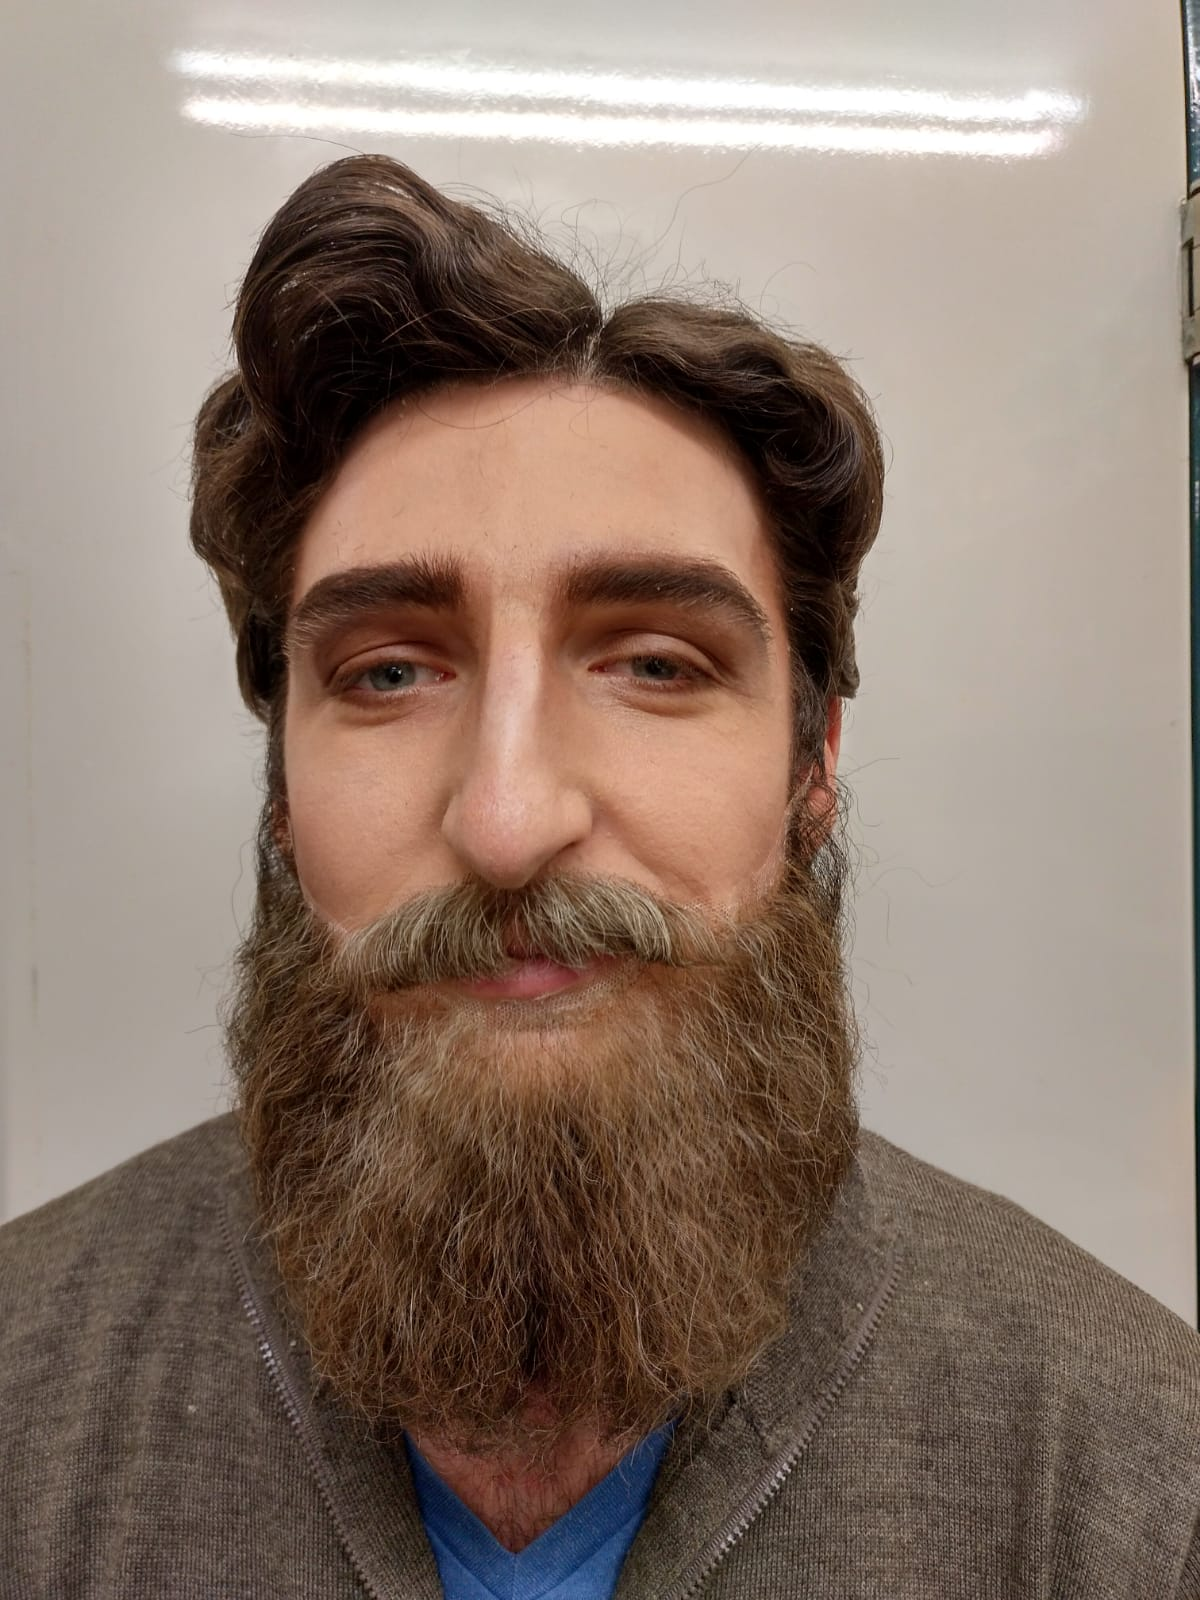
\includegraphics[scale=0.1]{./images/Penner}
    \caption{Caption}
    \label{fig:my_label}
\end{figure}

-------------------------------------------------------------------------------------------

\section{Eignung von Mehrwegverpackungen für typische Bauprodukte und Baustoffe}
\label{sec:Eignung von Verpackungen von Bauprodukten und Baustoffen:Eignung von Mehrwegverpackungen für typische Bauprodukte und Baustoffe}

%Die Eignung von Mehrwegverpackungen hängt stark von den Eignungskriterien ab. also die erst machen bzw sich überlegen welche es sein könnten.

Typische Bauprodukte und Baustoffe: (Definition)
%-->darauf referenziert die Eignung von MEHRWEGverpackungen
-abhängig von den Anforderungen
typische Bauprodukte und Bautoffe (unabhängig von der Verpackung) wählen:
    
    -Aufbau nach Baubetrieb:
    -Rohbau:
        -Aushub(Erde)
        -Beton
            -Betonabstandshalter
            -Fertigteile aller Art
            -Bei Ortbeton:
                -Wasser
                -Zement
                -Steine/Kies(Grob- und Feinkorn)
                -Sand
                -zusatzstoffe und -mittel
        -Stahl
            -Bewehrung
        -Rohre(Entwässerung
        -Dämmung
            -Dämmwolle (Mineralfaserwolle, etc)
            -Styrodur(synthetische Dämmung?)
        -Folie(zum schutz von Wassereintritt(im keller))
        -Bitumen (für den Keller)
        -Noppenfolie
        -Mauerwerk
            -Kalksandstein
            -Ziegel
            -Mörtel
            -Zement
            -Yttong(richtiger Name pls)
        -Holz
            -Sparren und Pfetten
        -Ziegel fürs Dach
        
        
        Brandschutzdecken und Gipsfaserplatten, Rahmenprofile und Ausgleichsschüttung
        -Dämmstoffe:
            -->Schall- oder Wärmedämmung, technische Isolierung von heizungen, fachgerechte Installation des Brandschutzes
        -Bauelemente:
            -->Fenster und Türen, Tore und Treppen
        -                    -Fassade
                        -->Vom Wärmedämm-Verbundsystem über Verblendmauerwerk und Außenputz bis hin zur Metall- oder Holzfassade
                        --> für private Wohnhäuser sowie für Gewerbe- und Industriegebäude
                    -Holz:
                        -->Unterbau: Für die Konstruktion von Dachstühlen und Wänden erhalten Sie bei uns Plattenware, Schnittholz und Co
        -Fliesen
            -verschiedene Materialien: zb Keramik, Naturstein(Steinzeug), Holz, Laminat, PVC, marmor, granit, quarzit, sandstein, terracotta
                -->Unterscheidung beim Transport und der Verpackung
        -Garten und Landschaftsbau:
            -betonplatten/betonfliesen vs natursteinfliesen
            -Zäune
                -Holzzäune, Maschendrahtzaun, WPC-Zaun(Wood Plastic Composite) =Verbundwerkstoff, Metallzaun
            -Pflastersteine
                -aus: Beton, Naturstein(zb Basalt), Hochofenschlacke, Beton mit Natursteinzusätzen
            -Terassendielen
        -Zierkies und -split
        -Holz
            -->Kantholz, Rundholz, Bauschnittholz, Holzplatten oder Holzbalken           -->Konstruktionsvollholz (KVH), Schnittholz, Schalungen und Bretter sowie Brettschichtholz (BSH) und Hobelware
            -->Holzkonstruktionen (Dachstühle; Nagelbinder,Holzrahmenbau), Holzwerkstoffe, Holzfaserdämmstoffe, Terrassenholz und Balkonbeläge
            -->Konstruktionsvollholz (KVH), Brettschichtholz (BSH), Hobelware, Sperrholz, Terrassen-Beläge, OSB-Platten, Spanplatten,  Holzdämmstoffe, sowie ein umfangreiches Sortiment an sägefrischem Schnittholz
        -Parkett, Laminat und Vinyl-Boden-->stukateur
        -Putz
        -Türen, Tore \& Fenster
        -Elektrikersachen
        -Heizungsbauer
            -Rohre und Heizung
        

    

gewisse Ordnung erstellen bzw in grobe Verpackungssysteme runterbrechen
    -->diese dann mit den Eignungskriterien koppeln und evtl sogar eine Art "Tabelle erstellen mit den Eignungskriterien auf der Abszisse und typischen Bauprodukten/Bauproduktverpackungen auf der Ordinate.
        
    
Die Eignung von Mehrwegverpackungen für typische Bauprodukte und Baustoffe ist abhängig von den Anforderungen an die Ware, die durch Verpackungen gewährleistet werden muss.

Als genutzt Mehrwegbehälter werden hier folgende ... genannt :

        Europaletten, sowie Pfandpaletten:
        %https://www.hausjournal.net/europalette-belastung :
            -Punktbelastung: 1000kg/1t
            -Flächenbeslastung: 1500kg / 1,5t; EPAL-Palette bs 2t(quelle eins drunter)
        -%https://www.vallee-partner.de/blog/paletten :
            -gefertigt aus Holz, Restholz, Kunststoffgranulat oder Recyclingkunststoffen (90 Prozent aus Holz),Plastikpaletten, Paletten aus Wellpappe, sowie Metall- und Papierpaletten
            -etwa 20 Prozent der gesamten Holzproduktion in Europa auf das Konto von Holzpaletten und -verpackungen
            -Holzpaletten werden vorwiegend aus Produktionsresten wie der Seitenware von Nadelhölzern gefertigt
            -Eine Europallette gilt als nicht mehr tauschbar und muss repariert werden, wenn beispielsweise Absplitterungen oder Brüche die sichere Nutzung gefährden oder Bretter, Klötze oder Markierungen fehlen.
            -Nicht mehr reparierbare und daher unbrauchbare Paletten, die die Reparaturprüfung nicht überstehen, werden meist in ihre brauchbaren Einzelteile zerlegt, welche wieder zu Paletten verarbeitet werden können. Die zerstörten oder morschen Teile werden im Schredder oder einer Entsorgungsanlage vernichtet; dies geschieht in eingetragenen, von der EPAL lizensierten Betrieben
            -Upcycling von EPAL Paletten ist noch ein thema auf das genauer eingegangen wird in der quelle.
            -für die lagerung und des transport, sowie be- und entladen
            -als untergrund für bigpacks
            -für Dachziegel
            -für betonprodukte
                -rohre,fliesen,L-shape, 
            -für eimer
            -für plastikkanalrohrsseme
            -zementsäcke
            -metalleinzelteile
                -stäbe
            -dämmung(aufgerollt)
            -Steine aller Art, die annähernd rechteckig sind
                -kalksandstein
                -yttong
            -als "Unterboden" für Gitterboxen und deren Transportware

        -gitterboxen/euroboxen /Boxpaletten
            -für rohre, loses material,für kleinere Steine
            -mit und ohne deckel erhältlich
            -für Kran oder nur Stapler geeignet
            -Sichert die Ware (auf einer Palette)
            -%https://de.wikipedia.org/wiki/Gitterbox
            -bietet die Möglichkeit des Stapelns von unförmiger Ware
            -Traglast (1000 bis 1500 Kilogramm),
            -die Auflast (4400 bis 6000 Kilogramm)
            -3-5 Stück stapelbar
            -->Möglichkeit einer Blocklagerung besteht
                -->bis zu sieben gestapelten Gitterboxen üblich(in der Blocklagerung)
            -Eigengewicht ca 70 kg
            -Anwendung bei instabilen und druckempfindlichen Güter (bei der Lagerung)
            -Die vorhandenen zwei Vorderwandklappen sind drehbar um eine waagerechte Achse gelagert. Die Klappen dienen der besseren Entnahme der geladenen Ware.
            -Es gibt auch faltbare Gitterboxen, die beim Rücktransport bis zu 80 Prozent Platz sparen
            -"Halbhohe Gitterbox" ist etwa halb so hoch, bei sonst gleichen Abmessungen
            -"Hohe Gitterbox" existiert(Höhe 1,8m)
                - Nutzvolumen von etwa 1,6 Kubikmeter und vorne eine Klappe
            -"Große Gitterbox"
                -bei doppelter Breite, bei sonst gleichen Abmessungen wie die hohe Gitterbox, ein Nutzvolumen von etwa 3,2 Kubikmetern. Auch sie hat eine Klappe vorne.
        Siehe auch:
            -DIN EN 13626, Verpackung – Boxpaletten – Allgemeine Anforderungen und Prüfverfahren:
            DIN 13626:2003:
                -Vorgesehen für die wiederholte Anwendung
                -behalten ihre gebrauchstauglichkeit und sichere handhabung
                -werden verwendet für: 
                    -mechanische Handhabung mit gabelstapler und Handhubwagen
                    -Massenlagerungen in stapellagern, bei denen es aus Sicherheitsgründen nicht ratsam ist, Boxpaletten bis zu einer Höhe zu stapeln, die das Siebenfache der kleineren horizontalen Abmessung der Boxpaletten überschreitet
                    -Transport
                -Diese Europäische Norm gilt für Boxpaletten, Rungenpaletten und Gitterboxpaletten, nicht aber für Silo- und
                -Sie können von fester Bauart, zusammenlegbar oder zerlegbar sein. Die Produkte, die in dieser Norm behandelt werden, sind Boxpaletten, die mit Gabelstaplern oder Hubwagen, nicht jedoch mit anderen Hebevorrichtungen gehandhabt werden können Tankpaletten
                -Boxpalette, Rungenpalette oder Gitterboxpalette
                    -entweder von fester Bauart, zusammenlegbar oder zerlegbar
                -verschiedene Lastrechnungen:
                    -Nennlast, Nennstapellast, dynamische Last, Prüflast
                -Anforderungen eine Gitterbox:
                    -muss mit Stapelvorrichtung versehen werden
                    -Handhabung vom Boden mit Gabelstapler/Hubwagen ermöglichen
                    -die Höhe der Boxpalette darf nicht das doppelte des kleinsten Bodenmaßes überschreiten
                -Prüfungen
                    -Prüflast: 2 Verfahren
                    -Klimatische Konditionierung:
                        -keine erforderlich für Boxen, wenn vollständig aus Metall
                -es gibt Kunststoffpaletten, Holzpaletten, Holzfaserpaletten
            -Europaletten, Container, Fahrzeug(Sattelauflieger) sind Transporthilfsmittel und damit Teil der Ladungsträger!
            
        -big bag/Bulk bag/ Jumbo bag/ FIBC(=Flexible Intermediate Bulk Container)
            (-überwiegend schüttmterial- kies, sand, ziersplit.)
            -Anwendungsbereich
                -feste Füllgüter in Pulver,- Granulat,- Pastenform
            -Arten von FIBC(BigBags)
                -flexible Großpackmittel(FIBC)
                    -bestehen aus flexiblem Material wie Gewebe, Kunststofffolie, Papier und sind so konstruiert, dass sie mit der Füllung in in Berührung kommen, entweder direkt oder durch einen Inliner, und im leeren Zustand zusammenfaltbar sind
                -Mehrweg-FIBC für hohe Beanspruchung
                    -ein FIBC, vorgesehen für eine Vielzahl von Befüllungen und Entleerungen, der sowohl beim Hersteller und/oder Anwender in einer Weise repariert werden kann, dass die Zugfestigkeit nach Reparatur mindestens so groß ist wie im Original
                -Mehrweg-FIBC für normale Beanspruchung
                    -ein FIBC, vorgesehen für eine begrenzte Anzahl von Befüllungen und Entleerungen
                    -arf im Falle einer Beschädigung nicht wiederverwendet werden, d. h., er ist nicht reparierbar
                    -Das Auswechseln eines herausnehmbaren Inliners wird nicht als Reparatur angesehen
                -Einweg-FIBC
                    -ein FIBC, vorgesehen für nur eine einmalige Befüllung
                -Nenntragfähigkeit (SWL)
                    -die maximale Last, die der FIBC laut Zertifikat im Einsatz tragen darf
                -FIBC.Teile/Komponenten
                    -Mantel
                        -ein ein- oder mehrlagiger Schlauch, der nahtlos oder aus einem oder mehreren Teilen zusammengesetzt ist
                    -Boden
                        -jener Teil des FIBC, der mit dem Mantel verbunden ist oder eine Einheit mit ihm bildet und die Grundfläche des stehenden FIBC bildet
                    -flacher Boden
                        -Boden ohne Öffnung
                    -Boden mit Öffnung
                        -flacher, konischer oder anders geformter Boden mit einer Öffnung
                    -ganz offener Boden
                        -Verlängerung des Mantelgewebes, das nach dem Verschließen den Boden des FIBC bildet
                    -Deckel
                        -der obere Teil des FIBC, ohne Hebevorrichtungen, der nach dem Verschließen den Deckel des FIBC bildet
                    -Körper
                        -der Mantel und der Boden des FIBC
                    -Inliner
                        -integrierter oder herausnehmbarer Behälter, der in den FIBC passt
                -Betriebsvorrichtungen
                    -Einfüllöffnung, Einfüllstutzen, Einfüllschlitz, Auslauf, Auslaufstutzen, Verschlüsse(Gurte, Seile, Riemen usw., die zum Verschließen der Einfüll- und Auslauföffnungen verwendet werden)
                -Handhabungsvorrichtungen
                    -Stütz und Hebevorrichtungen
                        -Gurte, Schlaufen, Seile, Ösen, Rahmen oder andere Vorrichtungen, die aus Verlängerung des Mantels des FIBC gebildet werden oder integriert oder abnehmbar am FIBC angebracht sind und für das Stützen oder das Heben des FIBC verwendet werden
                    -Aufhängung(Vierpunkt, Dreipunkt, Einpunkt)
            -Werkstoff:
                Die Eigenschaften der Materialien dürfen durch geeignete Zusätze modifiziert werden, um die Beständigkeit des Materials, z. B. gegen Schwächung durch Wärme und Sonnenlicht, zu verbessern und die Wirkung von statischer Elektrizität zu verringern.
            
        -container

-Ladeeinheit (LE)
    besteht aus: 
        -Ladehilfsmittel: z. B. Palette, Container, Tablar, Gitterboxpalette, Unit Load Device
        -Ladeeinheitensicherungsmittel
        -Packstück
    -Unterteilung in:
        -LE mit tragender Funktion: (Ladungsträger)
            -v.a. Paletten aus Holz, Kunststoff und Metall, aber auch:
                -Industriepalette, Rungenpalette, Rollpaletten, Einwegpaletten
            -Stapelung ist vierfach übereinander möglich
        -LE mit umschließender Form:
            -v.a. Gitterboxpaletten
                -bestehen aus:
                    -drei festen Gitterwänden, einer abnehmbaren Vorderwand,einer Bodenfläche (siehe Gitterboxen)
            -neben Gitterboxen gibt es noch:
                -Vollwandboxpaletten,
                -spezielle Klappboxen und Faltboxen
                    -->bieten beim Rücktransport eine Volumeneinsparung von 60 %
        -LE mit abschließender Form:
            -v.a. Container, aber auch  Wechselbrücken
    
       
------------------------------------------------------------------------------------------

\section{Potentiale und Herausforderungen verschiedener Mehrwegverpackungen}
\label{sec:Eignung von Verpackungen von Bauprodukten und Baustoffen:Potentiale und Herausforderungen verschiedener Mehrwegverpackungen}

%dieses kapitel gehört eigentlich zur Eignung von Mehrwegverpackungen. Hierbei sollen die potentiale identifiziert werden. Operator: Identifizieren.

hier eigentlich die verschiedenen Verpackungssysteme einfach hinschreiben die ich im Raab kercher gesehen habe(die mehrwegverpackungen eben)
    -->Einwegverpackungssysteme dann in das nächste Kapitel?

------------------------------------------------------------------------------------------

\input{sections/Ansätze von Systemen}



%% Dieser Teil der Arbeit soll die Arbeit abschließen. Ziel ist, die erarbeiteten Ergebnisse für den Leser zusammenzufassen und diese letztendlich kritisch zu betrachten und eventuell mögliche weitere Schritte kurz aufzuzeigen.





\chapter{Schluss}
\label{ch:Schluss}

-fasst die wichtigsten Ergebnisse prägnant zusammen und stellt somit den Höhepunkt deiner Bachelorarbeit dar

-steht im direkten Zusammenhang mit der Einleitung, da du auf die Forschungsfragen oder Hypothesen eingehst, die zu Beginn der Bachelorarbeit aufgestellt wurden

-Die Länge des Fazits ist abhängig vom Umfang deiner Arbeit, sollte jedoch ca. 5–10 Prozent der gesamten Bachelorarbeit ausmachen

-Keine neuen Informationen und Interpretationen
-Keine Beispiele und Zitate:
    -Im Fazit fasst du Fakten zusammen und erklärst sie nicht anhand neuer Beispiele und Zitate anderer Forschenden
-Dein Ergebnis ist immer wertvoll
    -Es kann vorkommen, dass deine Ergebnisse nicht deinen Erwartungen entsprechen. Wenn du deine Forschungsfrage aber gut gestellt hast, bspw. mit den Formulierungen ‚wie viel‘ oder ‚inwiefern‘, wirst du immer ein wertvolles Ergebnis erhalten, das die Forschung auf diesem Gebiet weiterbringt.
-Beim Präsentieren der Fakten verwendest du in einem Fazit das Präsens. Wenn du auf deine Forschung verweist, benutzt du das Präteritum.

-Elemente eines Fazits:
    -Abschließende Beantwortung deiner Forschungsfrage.
    -Gesamtdarstellung deiner wichtigsten Ergebnisse.
    -Zusammenfassung der Schlussfolgerungen aus dem Diskussionsteil (z. B. bezüglich offen gebliebener Fragen oder Ausblicke auf zukünftige Forschung).
-keine Elemente eines Fazits:
    -Wiederhole nicht nur Formulierungen aus deinem Hauptteil.
    -Sei nicht zu bescheiden, sondern zeige, was du erreicht hast.
    -Bringe keinen neuen Ideen, Studien oder Beispiele ein.
    -Schreibe das Fazit nicht kurz vor knapp, sondern nimm dir genügend Zeit.
    
-Unterschied zwischen Fazit und Diskussion

Oft kann der Unterschied zwischen dem Fazit und der Diskussion ein wenig verwirrend sein. Diese Tabelle schafft Klarheit und erklärt die wichtigsten Unterschiede:

Fazit:       
    -Zusammenfassung 	
    -Kurz und bündig 	
    -Gesamtdarstellung 	
    -Keine Beispiele und neuen Informationen 	

Diskussion:
    -Interpretation
    -Ausführliche Behandlung der Resultate
    -Evaluation
    -Beispiele und neue Informationen

-------------------------------------------------------------------------------------------

\section{Fazit/Zusammenfassung der Kernthese}
\label{sec:Schluss:Fazit/Zusammenfassung der Kernthese}

\section{Schlussfolgerung}
\label{sec:Schlussfolgerung}

\section{kritische Würdigung}
\label{sec:kritische Würdigung}

\section{Ausblick}
\label{Ausblick}


auch evtl einen Ausblick auf eine weitere anschließende bachelorarbeit
        - wo wrde diese anschließen
        -welche fragen/problemzonen könnte man darin behandeln?

%% --------------------
%% |   Bibliography   |
%% --------------------

%% Add entry to the table of contents for the bibliography
\printbibliography[heading=bibintoc]

%% ----------------
%% |   Appendix   |
%% ----------------
\appendix





%In den Anhang der Arbeit werden diejenigen Teile gestellt, die aufgrund ihres großen Umfanges den Textteil sprengen würden, jedoch für das Verständnis von Relevanz sind. Der Anhang ist lediglich eine Ergänzung zum Text in Form von Übersichten, Tabellen, Fragebogen oder Grafiken. Erläuterungen haben im Anhang nichts zu suchen.
%Bei mehreren Anlagen sollte aus Gründen der Übersichtlichkeit ein extra Inhaltsverzeichnis der Anlage vorangestellt werden.





{\chapter{Anhang}}
\label{chap:Anhang}


%% -------------------
%% | Example content |
%% -------------------
\section{ökologisch abbaubare Einwegverpackungen als Alternative zu konventionellen Einwegverpackungen}
\label{sec:Anhang:ökologisch abbaubare Einwegverpackungen als Alternative zu konventionellen Einwegverpackungen}
		
%\setcounter{figure}{0}
		
%\begin{figure} [ht]
%  \centering
%  \caption{A figure}
%  \label{fig:anotherfigure}
%\end{figure}






\begin{acronym}

\acro{zb}[z.B.]{zum Beispiel}

\end{acronym}


\end{document}
